%   *******************************************************************
%   * THIS IS THE MAIN FILE--RUNNING LATEX ON "AllegThesis.tex" WILL  *
%   * GENERATE THE ENTIRE THESIS (ASSUMING YOU HAVE NOT RENAMED IT).  *
%   * IF YOU ARE USING BIBTEX, RUNNING BIBTEX ON "AllegThesis" SHOULD *
%   * GENERATE YOUR BIBLIOGRAPHY. SPECIFIC DETAILS DEPEND ON WHAT     *
%   * ENVIRONMENT AND TOOLS YOU ARE USING (E.G., TEXMAKER OR COMMAND  *
%   * LINE TOOLS LIKE PDFLATEX OR ...).                               *
%   *******************************************************************
%
% AllegThesis.tex
% by A. Thall
% 13 Feb 2003
%
% Revised by R. Roos
% Nov 2013
%
% This document provides a sample Senior Thesis template for use
% by students in Allegheny's CS and Applied Computing programs.
%
%   *******************************************************************
%   * LOOK FOR BLOCK COMMENTS SUCH AS THIS ONE FOR AN EXPLANATION OF  *
%   * THIS DOCUMENT AND HOW TO MODIFY IT FOR YOUR OWN THESIS!         *
%   *                                                                 *
%   * ANY LINE BEGINNING WITH A "%" IS A LATEX COMMENT AND IS IGNORED *
%   * BY THE LATEX PROCESSOR. YOU ARE ENCOURAGED TO COMMENT YOUR OWN  *
%   * LATEX CODE TO HELP YOU REMEMBER WHY YOU DID THINGS A CERTAIN WAY*
%   *******************************************************************
%

%   ********************************************************************
%   * THE FIRST SECTION OF THE MAIN LATEX FILE IS THE "PREAMBLE." IT   *
%   * INSTRUCTS LATEX TO IMPORT SPECIAL PACKAGES FOR THINGS LIKE       *
%   * INCLUDING FIGURES, DOUBLE-SPACING, COLORED TEXT, ETC.            *
%   * DEPENDING ON YOUR NEEDS, YOU MAY FIND IT NECESSARY TO USE PACK-  *
%   * AGES THAT ARE NOT INCLUDED IN THIS TEMPLATE. SIMPLY IMITATE THE  *
%   * "\usepackage{...}" COMMANDS SHOWN BELOW.                         *
%   ********************************************************************

%   ********************************************************************
%   * BEGINNING OF PREAMBLE:                                           *
%   ********************************************************************

\NeedsTeXFormat{LaTeX2e}
\documentclass[12pt]{report}

%   ********************************************************************
%   * ALL BUT ONE OF THE FOLLOWING 5 LINES SHOULD BE COMMENTED OUT.    *
%   * (NOT ALL OF THESE OPTIONS HAVE BEEN TESTED IN THIS REVISION!)    *
%   ********************************************************************

%\usepackage[debug,draft,double]{gatorthesis} % for student proof doublespace
\usepackage[bottom,double]{gatorthesis} % for final department copy
%\usepackage[debug,draft,single]{gatorthesis} % for student workcopy
%\usepackage[single]{gatorthesis} % for student
%\usepackage[debug,draft,nolists,nofront,single]{gatorthesis} % more options


\usepackage{comment}     % provides a way to "comment out" sections in blocks
\usepackage{doublespace} % final document should be double-spaced!
\usepackage{amsmath}     % special symbols
\usepackage{amssymb}     % more special symbols
\usepackage{epsfig}      % needed for including figures
% \usepackage{fancybox}  % --- DISABLED BY RSR, SEP 2013 ---
\usepackage{url}
\usepackage{listings}
\usepackage[figure]{algorithm2e}
\usepackage{graphicx}

%   ********************************************************************
%   * OPTIONAL: IF YOU WANT VERY FINE CONTROL OVER HOW LATEX HYPHENATES*
%   * CERTAIN WORDS, YOU CAN PUT WORDS IN A "\hyphenation" COMMAND AS  *
%   * SHOWN IN THE FOLLOWING EXAMPLE. OTHERWISE, YOU MAY JUST IGNORE   *
%   * THE NEXT COMMAND.                                                *
%   ********************************************************************

% EXAMPLE: Don't hyphenate the words "itself" or "linear". Hyphenate 
%          "representations" only at the places indicated by the "-":

\hyphenation{itself repre-sen-tations linear}

%   ********************************************************************
%   * THE FOLLOWING COMMAND HAS BEEN DISABLED--IGNORE.                 *
%   ********************************************************************
% The following provides a box to surround the thesis statement
%\newenvironment{Thesis}%
%{\begin{Sbox}\begin{minipage}{.95\linewidth}}%
%{\end{minipage}\end{Sbox}\begin{center}\fbox{\TheSbox}\end{center}}

%   ********************************************************************
%   ********************************************************************
%   ***  END OF PREAMBLE.                                            ***
%   ********************************************************************
%   ********************************************************************



%   ********************************************************************
%   * DOCUMENT CONTENT STARTS AT THE "\begin{document}" COMMAND:       *
%   ********************************************************************

\begin{document}

%   ********************************************************************
%   * FILL IN THE "{...}" BELOW WITH YOUR INFORMATION.                 *
%   ********************************************************************

\thesistitle{Optimizing Traffic Flow with a Genetic Algorithm}

\thesisauthor{Adam Wechter} \thesisadvisor{Dr. Gregory Kapfhammer}

\thesisnumber{CS14-15} % SEE PAULINE LANZINE TO GET YOUR REPORT NUMBER!

\thesisreadera{Dr. Janyl Jumadinova}


%   ********************************************************************
%   * IN RARE CASES YOU MAY HAVE MORE THAN TWO READERS, IN WHICH CASE  *
%   * YOU SHOULD UN-COMMENT THE FOLLOWING AND ADD NAMES:               *
%   ********************************************************************
% \thesisreaderb{Dr. Your Thirdreader} 
% \thesisreaderc{Dr. Your Fourthreader}
% \thesisreaderd{Dr. Your Fifthreader}

%   ********************************************************************
%   * YOU MAY IGNORE THE FOLLOWING COMMAND:                            *
%   ********************************************************************
%%\date{\FileRevised \\ $\mbox{}$Revision: 1.8 $\mbox{}$}

\thesismaketitle         % Creates the title page
\thesismakecopyright     % Creates the copyright page

%   ********************************************************************
%   * YOU MAY SPLIT YOUR THESIS INTO SEVERAL FILES AND "\include" THEM *
%   * AS SHOWN BELOW. FOR INSTANCE, FILE "abstract.tex" CONTAINS THE   *
%   * ABSTRACT, FILE "ack.tex" CONTAINS THE ACKNOWLEDGMENTS, ETC. YOU  *
%   * MAY, OF COURSE, PUT EVERYTHING INTO ONE HUGE FILE, BUT THERE ARE *
%   * ADVANTAGES TO SPLITTING THINGS UP--FOR EXAMPLE, YOU CAN COMMENT  *
%   * OUT "\include" LINES OF SOME PARTS IN ORDER TO PRINT DRAFTS      *
%   * CONTAINING SELECTED SECTIONS OF YOUR THESIS, SAVING PAPER AND    *
%   * PRINTING COSTS.                                                  *
%   *                                                                  *
%   * YOU ARE NOT REQUIRED TO HAVE A "dedication"--IF YOU DON'T, JUST  *
%   * DELETE THAT LINE OR COMMENT IT OUT WITH A LEADING "%"            *
%   ********************************************************************

\begin{abstract}

Traffic gridlock and delay waste precious resources and is known to be  worsening as populations increase.  This makes alleviating the problem all the more important and drives research to find new, novel techniques to address the many causes of traffic congestion.  This paper offers an evolutionary algorithmic approach to optimizing traffic control devices at intersections to feasibly and affordably reduce total time transit, total time delay, and total fuel consumption of the vehicles.  Extensive configuration trials suggests that this process can contribute to optimize a given system, and points  to future study and modification of these types of algorithms on larger and more realistic city plans. This research delivers a simple, ideal, discrete event simulator, which is able to solve for fitnesses of a traffic system with a user-defined traffic control system configuration, as well as the customized ECJ engine which solves for the highest fitness using the simulator as the evaluator.
\end{abstract}
  % REQUIRED!

\begin{dedication}

I'd like to thank, firstly, my professors Kapfhammer, Jumidanova, Roos, and Cupper, for the help they provided me guiding and sparking the interest and passion I hold for programming today.  My mother and father, for being there through the most rewardingly difficult years of my education, as well as my brothers for releasing the tension when it was needed most.  If it weren't for my family, I would never have even made it to the comp so for their drive, I am grateful.  I'd also like to thank my dear friends BJ Nelson, who was a constant pressure and egging on helped me preserveer, Katherine Murray, who's friendship and sense of humor got me through the days, and finally Bridgette McCauley, who always believed in me.
\end{dedication} % OPTIONAL

\include{ack}       % OPTIONAL, BUT ALMOST EVERYONE INCLUDES IT

%   ********************************************************************
%   * FRONT MATTER--TABLE OF CONTENTS, ETC. YOU PROBABLY DON'T NEED TO *
%   * CHANGE ANY OF THIS UNLESS YOU HAVE NO TABLES OR FIGURES, OR YOU  *
%   * WANT TO CHANGE NUMBERING DEPTH FOR SUBSECTIONS, OR ...           *
%   ********************************************************************

\setcounter{tocdepth}{2}    % # of section levels shown in table of contents
\setcounter{secnumdepth}{3} % # of numbered subsection levels in the text

\tableofcontents
%\listoftables       % OMIT THIS IF YOU DON'T HAVE ANY TABLES
\listoffigures      % OMIT THIS IF YOU DON'T HAVE ANY FIGURES

%   ********************************************************************
%   * A GLOSSARY IS ALMOST NEVER NEEDED UNLESS YOU HAVE AN UNUSUALLY   *
%   * LARGE NUMBER OF SPECIAL TERMS OR NOTATIONS AND IT WOULD DETRACT  *
%   * TOO MUCH FROM THE FLOW OF THE PAPER TO DEFINE THEM IN-LINE.      *
%   ********************************************************************
%\include{glossary}  % OMIT THIS IF YOU DON'T HAVE A GLOSSARY (FEW PEOPLE DO)


%   ********************************************************************
%   * THE FOLLOWING "lstset" COMMAND IS ADAPTED FROM ONE FOUND AT:     *
%   * http://tex.stackexchange.com/questions/115467/                   *
%   * listings-highlight-java-annotations                              *
%   *                                                                  *
%   * SEE CHAPTER 3 AND APPENDIX A                                     *
%   ********************************************************************

\lstset{
  basicstyle=\footnotesize\tt, % the size of the fonts that are used for the code
  breakatwhitespace=false,     % automatic breaks only happen at whitespace?
  breaklines=true,             % sets automatic line breaking
  captionpos=b,                % sets the caption-position to bottom
  frame=single,                % adds a frame around the code
  language=Java,               % the language of the code
  keywordstyle=\bf,
  showspaces=false,
  showstringspaces=false,      % underline spaces within strings only?
  showtabs=false,
  tabsize=2                    % sets default tabsize to 2 spaces
}

%   ********************************************************************
%   * NOW INCLUDE THE CHAPTER FILES; COMMENT OUT ANY YOU DON'T WANT TO *
%   * PROCESS IN A PARTICULAR LATEX RUN.                               *
%   *                                                                  *
%   * INCLUDED FILES ARE ASSUMED TO END IN ".tex", E.G.,               *
%   * "ch01_overview.tex", "ch02_relatedwork.tex", ETC.                *
%   ********************************************************************

% ch:intro
%
% $Id: ch01_overview
%
%   *******************************************************************
%   * SEE THE MAIN FILE "AllegThesis.tex" FOR MORE INFORMATION.       *
%   *******************************************************************

\chapter{Introduction}\label{ch:intro} % we can refer to chapter by the label

%   ************************************************************************
%   * In LaTeX, new paragraphs are begun by simply leaving a blank line in *
%   * the LaTeX file.                                                      *
%   *                                                                      *
%   * The \\ characters should NEVER be used to end a paragraph.           *
%   * They are used only for inserting line breaks in certain situations.  *
%   *                                                                      *
%   * "Widows" (ending paragraph lines at the top of a new page) and       *
%   * "orphans" (opening paragraph lines at the bottom of a page) should   *
%   * be eliminated; this sometimes requires re-writing some of the        *
%   * text to change the line lengths.                                     *
%   ************************************************************************

This chapter will overview the entirety of the project including motivation for research, thesis statement, goals of the project, contributions of this project, and finally a general outline to the format and construction of this paper.  Primary and secondary sources are reserved for chapter \ref{ch:relatedwork} and will not be found in this section.  Also, this segment will begin to introduce some of the language and definitions that the reader will find necessary to understand the entirety of this paper, however rarely used terms will be defined within their respective section if they are not commonly used.  


\section{Motivation} \label{sec:motivation}
%Talk about problems related to traffic
% multi objective function
%how many cars per road

Traffic gridlock and delay waste precious natural, financial, and time resources, while contributing to local air pollution and global greenhouse gas accumulation.  It is well established that this problem is worsening is well-established.  Improved mass transit, increasingly fuel- efficient vehicles, and flexible work hours all have their places in addressing traffic gridlock and delay.  Approaches to traffic intersection control itself are also being created, tested, evaluated, and implemented as potentially promising large-scale palliative solutions.  The successful use of genetic algorithms in providing more optimal solutions to such problems as time tabling, scheduling, and other NP-Hard problems, and to some extent to the problems of traffic flow, supports expanding their use to further ameliorate traffic congestion.  Traffic intersection control and genetic algorithms (GAs) are two subjects of deep personal interest to the author, and the notion of combining those interests to address a major problem motivates this research.  

Of all the means of limiting the sequelae of traffic congestion, the most feasible and affordable in the short run is implementing traffic pattern changes through intersection control, using a system that minimizes investment in hardware and related equipment and their installation. Proposed systems that rely on universally installed internal automobile technology fail those criterion mentioned. Similarly, for reasons of cost alone, the ideal of restructuring an entire urban system and thus physically optimizing or overhauling the existing system is an essentially impossible one for existing cities.
 
Genetic algorithms (GA) are search heuristics which emulate natural selection and evolution to generate solutions to optimization or search problems; they are part of a larger collection of algorithms called evolutionary algorithms (EAs).  Fundamental to these algorithms is their uses of genetic representations to describe solution domains, in this case  binary arrays, as well as fitness functions that assign  numeric representations to the quality of the performance of solution domains.  Motivations for choosing this sort of algorithm for the process of optimizing traffic intersection configurations are threefold:  first of all, GAs have been successfully implemented in the past for two specific types of problems with great success, namely time-tabling and scheduling.  Both of these problems are known to be NP-Hard, which indicates that there are no known algorithms to effectively find  solutions in polynomial time.  Since traffic system optimization problems fall under similar constraints, genetic algorithms would seem to be a choice method for generating possible optimized configuration networks for traffic control.  Secondly, the success of several other projects involving implementation of genetic algorithms encourages further exploration and study.  Lastly, although many systems, such as the Sydney Coordinated Adaptive Traffic System (SCATS), work very well in real time, their development relies on initial layouts and timing configurations as standard starting points; determining those is already an expensive and time-consuming process.  Using GA-determined configurations to establish the standard starting points may reduce the time and costs involved  and thus encourage  more widespread use of these expensive  but proven systems.

\section{Thesis Statement}\label{sec:thesis}

Using a discrete event simulator as a testing and metric environment, it will be demonstrated that genetic algorithms are able to improve several benchmarking criteria, including decreasing time transit and time delay, while operating within the constraints of a realistic traffic experience. 

\section{Goals of the Project}\label{sec:goals}

This project has several goals primarily involving the creation of different components of the simulator and ECJ engine, followed by a series of objectives normally associated with empirical research.  By running custom or randomly generated grid designs and gathering critical data, the simulator will enable determination of the fitness of the current traffic network setup, as well as gathering information about vital information for comparison with a previous iteration.  Developing the simulator was the primary focus of this comprehensive project as subsequent phases depended on its functioning.

The next deliverable of this project involves the implementation and customization of the Java Evolutionary Computational genetic algorithm (ECJ).  ECJ is a dynamic, open source, freeware algorithm, which has been proven to efficiently and effectively solve stochastic optimization problems, more specifically ones involving metaheuristics.  Stochastic optimization is a class of techniques that use randomness to a degree in order to find the closest to optimal, and sometimes optimal, solution to NP-Hard problems.  Metaheuristics are strategies used to guide a search process using heuristics to find a good enough solution to some sort of problem.  Since metaheuristics are not problem specific, this project utilizes the framework provided by ECJ, along with the highly documented instruction manual to develop the algorithm described later in chapter \ref{ch:method}\cite{GAMANUAL}\cite{otherBook}. 

Only after the completion of these major components can the final objective of this project be attempted:  to execute the program in a series of tests and analyze the results from different scenarios.  The downside to GAs is that ``better" solutions are only in the realm of other solutions.  This being said, GAs are generally compared to different optimization algorithms for analysis, such as a completely random solution-generating algorithm that essentially brute forces a solution, saving the best found every iteration.  By comparing how the GA performs to some other algorithm, the reader will be able to easily judge its performance as a traffic control configuration optimizer.    

\section{Contributions}\label{sec:contributions}
The contributions of this senior comprehensive project include several promising new advancements to traffic systems optimizations.  Firstly, this paper will demonstrate through its results that the implemented genetic algorithm has, to a degree, successfully improved and optimized a idealized grid.  Additionally, there will be the beginning and basic framework of a traffic grid simulator which will allow for the testing and optimization of future traffic systems.  Finally, this paper will suggest improvements that future work could make to this study for a more successful configuration optimization.

\section{Thesis Outline}\label{sec:outline}
Chapter \ref{ch:relatedwork} reviews a number of past works in traffic control optimization and addresses their strengths and weaknesses.  It also covers basic information on genetic algorithms.  Chapter \ref{ch:method} outlines the method of approach used to establish the
results including details on the simulator and ECJ configuration.  This chapter also discusses threats to validity and details pertaining to the techniques used for testing.  Chapter \ref{ch:implem} contains details as to the results of testing and draws conclusions based on those results.  Chapter \ref{ch:conclusion} discusses the possibility of future work and reviews some of the different aspects covered in this project. % Introduction -- of course, you can name it anything!

% ch:relatedwork
%
% $Id: ch02_relatedwork
%
%   *******************************************************************
%   * SEE THE MAIN FILE "AllegThesis.tex" FOR MORE INFORMATION.       *
%   *******************************************************************
\chapter{Related Work}\label{ch:relatedwork}

\section{Secondary Sources}

\subsection{SCATS}
The Sydney Coordinated Adaptive Traffic System (SCATS) is one of the most commonly used traffic monitoring and regulating systems used today and has been deployed in 154 cities across 25 different countries, though under different names.  It was developed in late 1979 by A.G. Sims and K. W. Dobinson and was used primarily on major arteries in urban environments.  It is a dynamic on-line and real-time system which manages the timing of signal phases of different intersections to find the best fitting solution for the current traffic situation.  It also allows and incorporates real-time pedestrian traffic flows, public vehicle transportation, as well as public vehicle priority systems.  The priority system is generally associated with the tram and bus system where there are  high, medium, and low priority levels, with  low priority vehicles waiting their turn, while high priority vehicles skip all other phases to get to their call locations.  The system supports three levels of control as well, a local level, a master level, and the control center.  The control center is the central computer hub, which supplies all area-based traffic control and urban based traffic control(UTC) with information it keeps in its logs, and allows the entire system to be monitored from a central location with a holistic view of the system.  The master level is one level below that and is in charge of regional areas; it has a small amount of local storage for data as well as a control system and a logging system.  Finally, the lowest level of control is given to the local controller, which consists of a road side box at each intersection. These boxes contain the hardware to control the nearby intersections and allow for emergency updates as well as immediate control over particular intersections.  All of these different sections of the system are in constant communication with each other through the telephone lines, resulting in a robustly dynamic system\cite{SCATS}.

The drawback to this system is that it requires the purchase and installation of a large amount of hardware for the system to be implemented.  Back in 1980, when the paper was written, the cost of installing a system, not including the additional costs associated with rerouting traffic, etc., averaged 2.5 million dollars.  Additionally this system has an associated monthly cost for the use of the telephone wires, which the researchers estimated would be about  220 thousand dollars a year.  Further,  this system cannot be implemented immediately due to the fact that the city must take the time to install it\cite{SCATS}. 

This system boasts a 20 percent reduction in accidents and 20-48 percent reduction in delays, leading to an estimated 10 million dollars in fuel savings, and an 18 percent reduction in carbon monoxide(CO) emissions.  One of the final benefits that these researchers saw in their implementation was related to directing the preferred traffic flow of commuters.  They argued that by reducing delays and traffic congestion on the main arteries of routes into and out of popular areas, commuters were more likely to take the intended routes.  This in turn caused a reduction of impatient commuters attempting to cut through neighborhood areas in order to escape the delays associated with the main routes \cite{SCATS}.
	
\subsection{Vehicle-to-Vehicle}
Another recent topic of research in the field is the change from physical control devices to virtual, in-car devices, relying entirely upon the surrounding vehicles to gather data about the state of the intersection and to make timing decisions.  Research was presented in 2010 by Ferreira, et al.\cite{V2V} as a solution to overcome several problems which other traffic control systems have, such as the SCATS traffic system.  The researchers cite that the motivation behind this study lies within the problems that traditional traffic methods have, and introduce through its simplicity of sensor systems.  They say that the sensors in these physical systems, allow the controlling computers to make intelligent decisions based on their observations, however introduce the problem naivete of the rest of the environment, which can lead to possible large miscalculations of the actual state of the intersection.  For example, if the sensors which decide the length of the queue are only 200 feet back from the light, if a car is on that sensor, there is a chance that the queue goes beyond that distance and extends for a significant distance\cite{V2V}.  

To remedy this, the authors propose a traffic control system that is completely encapsulated within the car, from data collection, to decision making, and control signal indication, acting as a completely self-organized system.  Ferreira et al. make the assumptions that firstly, all of the vehicles in the system are equipped with a dedicated short range communication (DSRC) device, tuned to a specific channel so that the cars will be able to find each other, the cars are equipped with an up to date roadmap and accurate global positioning system (GPS), and some sort of dedicated Application Unit (AU).  The step process that this system proposes to implement involves firstly, establishing a Virtual Traffic Light (VTL) protocol with all the surrounding cars approaching the intersection to indicate that a traffic signal will be used at the upcoming intersection.  Following this step, the vehicles approaching the intersection are responsible for electing a leader node, which will be responsible for creating the VTL and broadcast the traffic light message to all surrounding node, as well as be responsible to serve as the primary form of infrastructure for that instance of the intersection.  This leader is elected using a predetermined algorithm so that there is no conflict; however, two rules apply to this leader node.  First, it must be stopped at the intersection and remain there while it is leading that intersection, and second, it must be the closest to the center, or front, of the queue in its lane.  This second criteria is strictly there to optimize communication.  Following this, the leader will broadcast the lighting signals to all nearby vehicles on an individual basis, which is why an accurate GPS is required in order to ensure that vehicles are correctly interpreted as to lane location.  The researchers conducted several simulations based on the major city of Porto, Portugal, and concluded that there was a significant benefit and case for viability\cite{V2V}.  While this system is a fascinating one, the researchers also made it clear that this system should primarily be used where traffic lights are not necessarily required, and that it should supplement the existing system.  Additionally, this research presumed that all of the vehicles in the environment are outfitted with specific hardware to allow this sort of communication to work.  Even if this were to be the protocol for a country, there are still several issues that could arise.  For example, if some country in Europe were to adopt this system and implement it completely as a substitute for the physical system, if any other vehicle from some outside country were to come into the nation, there is a chance that their car may not have the hardware to support it.  This could result in car accidents and other forms of delay for the entire system.

\subsection{Vehicle-to-Infrastructure}
In the case that a city does not wish to completely replace its existing system, there are cases where the idea of a real-time, intelligent system which uses information it gathers from nearby vehicles, instead of the environment like the SCATS case, to allow a traffic controller to make enlightened decisions about the signal selections.  Vehicular Ad-Hoc Network (VANET) is a very commonly explored technology which is used to collect and interpret information about nearby cars' speeds and positions.  Avzekar and Moon, 2014\cite{V2I}, propose a system which will use this VANET technology to interpret and gather information about the density of traffic approaching an intersection, and to make intelligent decisions about regulating this traffic; while favoring emergency vehicles, allowing them to run lights or giving them direct routes to their destinations.  The premise of this system is encapsulated in \ref{Figure 1}, which illustrates exactly how the system will work.  Note that in the diagram below, the RF receiver stands for a radio frequency receiver.
\begin{figure}[h]
	\centering	
	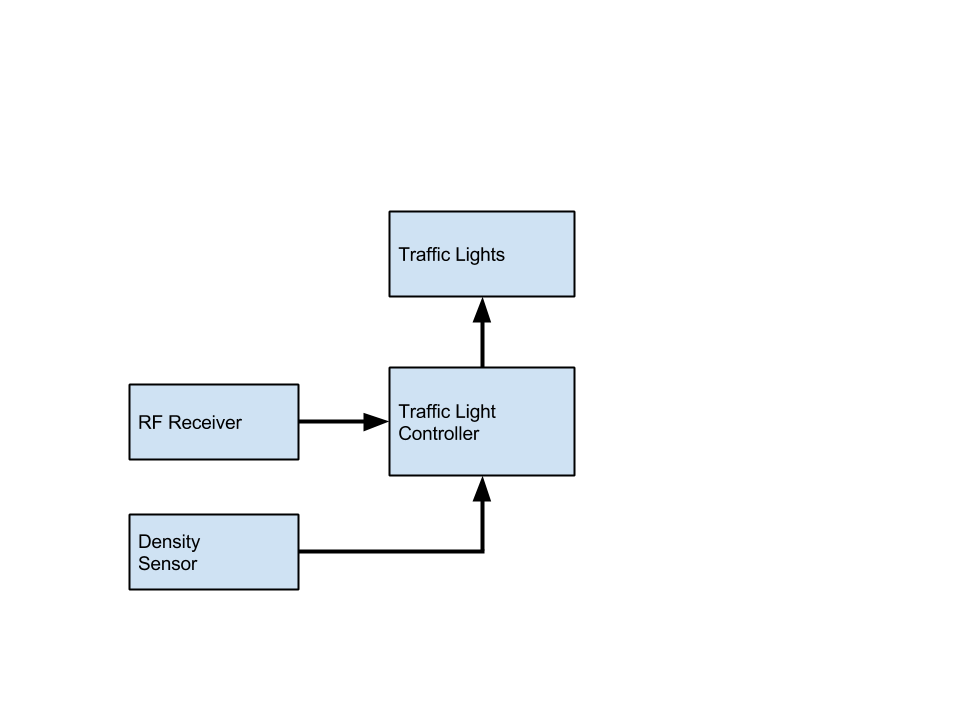
\includegraphics[scale=.4]{images/vanet.png}
	\caption{Block diagram of adaptive traffic system equipped with VANET}
	\label{Figure 1}
\end{figure}
The first methodology proposed by these researchers deals with optimizing traffic light timing based on the volume and density of the incoming traffic.  Using VANET, they make the case that they will be able to manage the system and to allocate greater time to higher flow streets at an intersection and significantly less time to lower density streets.  This is logical and generally the goal of any optimization of traffic control system.  The second goal of their implementation is one of greater interest, however, and deals with the priority system for emergency vehicles.  They propose that a city's emergency vehicles be outfitted with radio frequency transmitters to communicate with the traffic light controller as needed.  In this situation, all other nearby lights besides those in the emergency vehicle's lane will be immediately turned red until that ambulance, fire truck, or police car passes, after which the lights will resume their regular operation.  Using simulations, Avzekar and Moon were able to see that this approach to solving the traffic problem had no negative effects and resulted in consistent, smooth traffic flow.  However, by failing to make a cost-benefit of the VANET system, they render their research slightly inconclusive\cite{V2I}.  There are problems with this system that are not make mention, yet are definitely present.  First, VANET once again requires that \textit{all} vehicles in a system have certain pieces of hardware installed in order for the system to work.  Second, since security measures were not addressed, there is a chance that the radio frequency waves could be vulnerable to attacks. 

\subsection{Reinforced-Learning}
Although the previous examples of traffic optimization covered methods which used sensors and real time techniques in order to adequately manage systems, there are several ways in which a traffic system can be optimized through the use of algorithms.  One paper that showed promising signs of ways to optimize this system used collaborative reinforced-learning techniques in order to support many of the unpredictable aspects associated with urban UTC.  Salkham et al., 2008, propose using a collaborative reinforced learning system for the optimization process for several reasons, the most important being that reinforced learning is a great approach in unstable conditions where the flux of these systems are inevitable.  Further, using the collaborative method over the traditional method allows for the implementation to affect the decentralized aspect of traffic optimization. Through a comparative study, they were able to show that both the traditionally reinforced learning technique and the collaborative reinforced learning technique reduce average wait time per arrived vehicle; however, they noticed that the collaborative technique was able to improve the overall quality of the optimization.  Unfortunately, this study was done on a microscopic scale with regard to the simulation and detailed vehicles' behavior in a real city.  The microscopic aspect of the simulator signifies that it tracks vehicles moving around the network on a second or sub-second basis, making it very accurate after the initial ``warm-up" period.  Thus the study's are very promising and might, in fact, translate well to real world application\cite{CRL}.  


\section{Primary Sources}

Ceylan and Bell, 2004\cite{biGA}, cover two problems in one study: area traffic control optimization and user routing.  They present the problem as an equilibrium network design problem rather than as a scheduling problem.  Additionally, they call a known simulator named TRANSYT-7F to help evaluate the light timings of their genetically modified system.  The network used for this simulation is small having only six control junctures, or intersections.  Still, their findings are promising, suggesting that a genetic optimization can solve this type of problem.  They arrive at three major conclusions: first, that this process shows an improvement of around 34 percent by the 75th generation; second, that the solution is strongly affected by the initial set of timings; and third, that depending on the model, there can be a huge disparity in total optimization time, from 16.5 seconds to 18.4 hours\cite{biGA}.  The implication of these conclusions for the research project at hand is that flow patterns can be repeated multiple times with different initial traffic timings.  The traffic flow pattern the utilized were static, and tests were run multiple times with random starting traffic timing patterns determined by an algorithm.  This provided sufficient results to determine whether an optimization process failure was due to the traffic flow set-up, or by the initial starting values of that optimization run. 

Another example in which GAs not only worked but outperformed other stochastic algorithms is documented by Yun and Park, 2006\cite{CORISM}, in a paper on the application of optimization methods applied to an urban corridor.  They survey two existing optimization models for traffic timing, SYNCHRO(Husch and Albeck 2004) and CORISM.  CORISM is the most recent addition to the TRANSYT-7F model, which uses a microscopic model and includes three different heuristics: a GA, simulated annealing, and an optimization engine called OptQuest.   In their conclusion, the authors highlight that the recently introduced GA aspect of CORISM outperformed every other optimization method to which it was compared.  These include the other heuristics of CORISM, as well as the commonly used SYNCHRO.  While discussing future works, they caution future researchers that the performance of GAs is closely correlated to the original parameter settings.  Further, they warn that running these optimizations can be time intensive.  By showing that the GA outperformed the other heuristics by a rather large margin, around 15.2 percent in their measures of effectiveness, they influenced this researcher to focus on the implementations of a genetic algorithm rather than some other method\cite{CORISM}.

While the time and scope of this research paper do not permit the use of a multi-objective GA, there have been occasions where this method has been applied to traffic control configuration problems with some success.  One such example, completed by Li, Tao, and Chen, 2013\cite{moGA}, focuses on implementing a multi-objective GA on an oversaturated intersection.  The environment scale varied between one- and two-intersection environments.  Their study was motivated by the observation that many modern traffic control systems lack the ability to efficiently deal with circumstances where the amount of congestion overflows the normal boundaries.  The variables they identify include queue length, delay, cycle length, and others.  They determine that the number of variables, deems a multi-objective GA called NSGA-II to be the most appropriate approach.  Their study emphasizes the importance of having accurate and realistic simulators.  In their research, the authors were able to imitate several of the technologies available in real traffic systems, such as a NEMA controller.  In their conclusion they acknowledge the difficulties inherent in increasing the number of genes that the algorithm needs to consider; increasing the number increases the computational complexity of the problem and the associated time demands\cite{moGA}.  Additionally this study had no more than two intersections in any simulation which is incredibly small and leaves information wanting, for example, how oversaturated intersections in a UTC would be optimized by a genetic algorithm.   % Background, literature survey, ...

% ch:method
%
% $Id: ch03_thework.tex
%
%   *******************************************************************
%   * SEE THE MAIN FILE "AllegThesis.tex" FOR MORE INFORMATION.       *
%   *******************************************************************
% Fitness 153
\chapter{Method of Approach} \label{ch:method}
This chapter will discuss and present an overview of the programs used for this study.  It includes a detailed summary of the discrete event simulator, as well as descriptions of the ECJ tool used including parameter configurations.  It will also remark on details on the logic of why certain algorithms were used for different mechanisms as well as architectural decisions of the program.

\section{Test Environment}

This project has two major sub-projects comprising the performance testing environment, the simulator and the ECJ evolutionary algorithm suite.  The simulator has the sole purpose of receiving configurations of the light system, running a simulation based on a pre-determined traffic map, and evaluating the performance of an iteration and generating a correlating fitness value.  The ECJ package is in charge of the optimization of the overall system; it utilizes the fitness values to best judge which configurations are superior.

\subsection{Simulator}
%%%%%%%%%%  AROUND 585 FEET PER BLOCK!!!!!!!!!!
%%%%%%%%%%  Comment on accuracy vs continuous 
To begin with, this simulator is a discrete event simulator which takes four files and three ``modifier values'' as arguments and returns a fitness value based on several outcomes of this system, namely total time spent not moving at lights (time delay), total transit time, and approximate fuel used to travel through the system.  The simulator is an idealized environment in which accidents do not happen and cars react promptly to external environmental changes.  For example the cars react immediately to changes in traffic light color.  Furthermore, the entire system is within a perfect square grid; each road has the same length and the same speed limit.  Lastly, in this idealized system each road has two lanes, one in each direction.  This places constraints on cars being able to turn left if traffic flow is heavy.  The cars, as mentioned earlier, are relatively simplistic and all act the same way within the system.  Though variations of the different cars' rates of fuel consumption are possible, that option is not utilized.  The simplicity of this system is a result of time constraints and scale of scope; had more time and computing power been allocated, layers of complexity could have been introduced for better approximations of distances, staggered introductions of cars into the system, and non-grid patterned traffic maps.

As is, the simulator works in a way that mimics traffic rules and etiquette and uses seconds to mark the passing events.  Since this system is a discrete event simulation, using seconds to mark the passage of time allows for comparisons to be made in an accurate manner and allows easy access to the state of the system at any point that an action is performed.  Cars enter the system at the same time at the very beginning of the simulation, and after the specialized first move, which differs from all following actions for reasons explained later, the event lists are iterated through.   The car within the event then makes a decision regarding its movement then returns to the next list if it has not reached its final destination.  Following each iteration of car events, an iteration of node events is executed to update intersection states.  Time in the system is held in the individual cars as well as  in the nodes, allowing for easy manipulation of the state of the vehicle or the intersection lights.   This is because after a while, each intersection is on its own schedule.  The pseudocode shown in \ref{Traffic Simulator} is the basic process that the simulation follows by individually going through the car events and returning the events to the queue until each car reaches its destination and is removed from the queue.  Note that after the queue of cars is looped through, there is a secondary cleaning loop which resets the state of the car so that it can go again in the next rotation.

\begin{algorithm}[h]
 \SetAlgoLined
 \KwIn{Queue $CE \Longleftarrow Cars$}
 \KwIn{Queue $NE \Longleftarrow Nodes$}
 \KwResult{Fitness of intersection configuration} 
 \While{$CE$ not empty}{
  \For{$ce\in CE$}{
   \If{$c \in ce$ \emph{canGo}}{
    \eIf{$c$ at\_Destination}{
     remove from system\;
    }{
     \eIf{can\_it\_move} {
      try to move\;
      }{
      increment time values\;
     }
    }
   }
    {add $ce$ to $CE$\;}
  }
  \For{$ce\in CE$}{
   set \emph{canGo} true\;
  }
  \For{$ne \in NE$}{
   check\_and\_transition lights;
  }
 }
 \caption{Algorithm describing simulation process}
 \label{Traffic Simulator}
\end{algorithm}

Starting at the beginning, there are three files that are not reliant on the ECJ engine, unlike the configuration file.  These three files are the \texttt{node.txt} file, \texttt{edge.txt} file, and the \texttt{car.txt} file, which are comma-separated values to hold details about other aspects of the simulator.  The \texttt{node.txt} file contains information about the different nodes in the system.  The nodes are the heart of the simulator and at any given point, every ``car'' object in the system will be in one.  Nodes represent both intersections and roads connecting these intersections.  The \texttt{node.txt} file first supplies the overall dimensions of the grid, as well as the length of the roads in the grid, in feet.  The following lines of information provide the primary node data including whether the node is an intersection, in boolean format; the node ID, in form of \texttt{IorRxRowxColumn}, where the first value indicates whether it is a road or intersection while the other values represent a coordinate;  speed limit, in miles per hour; and an indicator as to intersection vs road, including type of road.  These final two merit further detail to describe what logic is used in the decision of their final forms.  The speed limit is an important aspect to measure time within the roads, however all intersections have a speed limit of 0 miles per hour.  This is because a car's location in the intersection is determined solely by other cars in the intersection and since real world intersections are often inconsistent in speed.  The final aspect of the nodes worth noting is the labeling of roads and intersections.  In order to easily determine lanes and the appropriate queues that cars enter when changing nodes, using the labels ``Lateral Roads'' and ``Vertical Roads'' made it significantly simpler than checking parts of the node IDs each time.  

The second file used was the \texttt{edge.txt}, which simply represents the connections that are drawn between the different nodes.  The file lists each connection once; however, when the information is brought into the system, the connections are doubled so that there is a link from node a to node b and vice versa.  These are primarily used when the cars decide directions.  After accessing these two files, the simulator can build a grid in which cars will be added.  Nodes are outfitted with directed queues to imitate cars moving in lanes.  These directed queues act as lanes; for example, North directional queues have cars moving from South to North.  While intersections have all four of these, the roads have only the two associated with their orientation, where lateral roads have the East and West queues and vertical roads have North and South queues.  Following the construction of the map, cars are added to the system.  The \texttt{car.txt} file contains first, the node ID of the car's starting position, as well as the node ID of the car's destination.  It is important to note that cars cannot start and end at the same node as that would lead to an infinite fitness value since the time of transit would be divided by a distance of zero.  The start and destination nodes are followed by the green-house gas emissions numbers, which are available on EPA's website.  This number, while available, is not utilized in this study; it is directly correlated to time within the system.  The next input data source is the cars' IDs, which are used primarily for debugging and quality control checks.  The final information is the cars' fuel consumption, in miles per gallon.  All of the variables that describe characteristics of the cars are used solely for calculation of the system's fitness after the simulation.

The final file that is used during the initiation process is the intersection configuration file.  This is read in from a comma-separated file format and is such that each line is a new intersection.  The intersections' configurations are in order and after the values are read in, the simulator iterates through the nodes and assigns each intersection the set-up determined by the ECJ engine.  All values of these chains are in binary, and the first digit indicates whether the intersection has a light or stop signs at the corners.  If the first value is a $0$, then the intersection has stop signs and the following 7 bits are of no consequence to the activity and behavior of the node.  However if the first value is a $1$, then there is a light at the intersection and the next three bits indicate the length of the North- South direction green light time.  If the decimal value of this number is $0$, then that light direction is automatically assigned the green light duration time of 15 seconds.  If it is not $0$, then the binary number is then multiplied by 15 seconds and is added to the initial 15 seconds value that is associated with a $0$ value.  The following three bits are also associated with the green light time, however, they refer to the East-West directional light.  The same rules as mentioned before apply to this value.  The final bit is used to indicate which direction has a green first, specifically, the North-South direction, indicated as true by a $1$ and false otherwise.

Once all of these outside values have been entered into the system, the car objects generate directions from their start nodes to their destination nodes.  This directions generation is provided by a breadth-first search algorithm which aims to create the route with the shortest path, regardless of the speed limit or any other factors besides distance.  Once this is done, the system is ready to begin and the cars are all individually loaded into separate car events and the nodes into the node events.  The first iteration of all of these events is more of a preliminary phase where cars are actually placed in the appropriate queues and the lights can begin rotating.  All cars immediately jump from their start nodes to their second nodes so there will be no problems in the future with directional queue decisions.  Additionally the internal car time variables are incremented as they normally would be.  The decision making behind updating which directional queue that a car belongs in requires the knowledge of the previous node. While this could have been randomly assigned for the first iteration,  some minor difficulties were averted by jump starting the system.  Once this happens, the car events are executed as they would normally be.  The first rotation for node events acts as it will for the rest of the simulation, incrementing the time variable as normal.

The car events execute in a simple way outlined by the pseudo code below.  It begins by checking if the car is in the system, and if it is, the simulator checks immediately if it is at its destination.  If the car proves to be at its destination, it is removed from the system and the details of the car's trip are recorded into the record data structures so they can be recalled later for calculation of the fitness value.  If the car is not at its destination, then it decides how to proceed, whether decisions should be made as if it is on a road, at an intersection that has a light, or an intersection that has a stop sign.  The simulator uses the time after the car leaves the system to do some cleaning of the queues to ensure no null values are displacing the lists, then replaces the car event back in the simulator to repeat these steps.  If the car is flagged as not being in the system, it will be removed from the list of car events thus reducing the size of the list until it is empty, marking the termination of the simulation.

\begin{algorithm}[h]
 \SetAlgoLined
 \KwIn{Car Event $CE$}
 \KwResult{Simulator with additional Car Event}
    \If{Car is in system}{
      \If{car at\_destination}{
       Exit system\;
      }
      \ElseIf{Car is\_on\_road}{
       Do road operations\;
      }{
      \If{Car is\_at\_light\_intersection}{
       Do light operations\;
      }{
       Do sign updates\;
      }
     }
     Re-queue car event to simulator\; 
    }{
    Do nothing, do not re-queue\;
    }
  \caption{Algorithm describes car event logic}
\label{Car Event}
\end{algorithm}

Light intersections and stop sign intersections work in different ways, one requiring information from the node, the other requiring information solely from the other queues at the intersection and the cars at the front of these ``lanes''.  The intersection this paper will review is the light intersection and is demonstrated in \ref{Light Intersection}.  The first principle is that lights have three states: green, red, or transition.  These first two are rather self-explanatory, where cars can go on green and must stop on red.  The transition period follows only after a green light and provides the opportunity for cars which wish to turn left, but did not have the opportunity during its green light because of traffic, to make that turn.  When a car arrives at the intersection, the first step it takes is to check whether or not it is allowed to move.  This is because in a situation where two cars at a green light, \texttt{car a} and \texttt{car b} where \texttt{car a} is at the front of the queue and \texttt{car b} is behind, if \texttt{car a} event is selected first and makes its movement into the next road. When \texttt{car b} is selected to make its decision and the car object decides to make a move because it is at the front of the queue and the light is green, there would be a conflict because two actions would be performed at the same time which in reality would cause a collision.  To prevent this conflict, each car has a boolean \texttt{can go} variable.  After confirming that the selected car is available for movement, the car checks the light signal and its logic branches.  If the appropriate directional lights are green, one of three possibilities will occur.  If the car is not at the front of the queue it will make no movement.  If it is at the front of the queue, it will proceed straight or right if either is its direction, or it will first check the oncoming lane and proceed left only if that queue is empty.  If the light is in a transition period, only if a car is at the front of the queue will it have the option of moving. If that lead car has a left turn to make, that left is given priority. If the lead car has a right turn, it will make it on the condition that the other lane across from it is empty.  After movement decisions are made, it is important to note that all of the other cars that are in the queue are immediately flagged as not allowed to go.

\begin{algorithm}
 \SetAlgoLined
 \KwData{Car $C$}
 \Begin{
  \If{Car can\_go}{
   \If{Light is\_green}{
    \eIf{Car not\_at\_front\_of\_queue}{
     Do nothing\;
    }{
     \eIf{Car going\_straight\_or\_right}{
      Update car info\;
     }{
      \eIf{Opposite queue is empty}{
       Update car info\;
      }{Do nothing\;}
     }
    }
   }                
  \ElseIf{Light is\_transition}{
   \eIf{Car moving\_left}{
    Update car info\;
   }{
    \eIf{Opposite lane Is\_empty}{
     Update car info\;
    }{Do nothing\;}
   }
  }
  \Else{Do Nothing\;}
  }
 }
 \caption{Algorithm describes light intersection logic}
\label{Light Intersection}
\end{algorithm}

\newpage
Sign intersections are slightly more complicated logically since in reality, various factors will often lead to behaviors that differ from that strictly dictated by law.  The simulation breaks down the intersection in a way that closely mimics the way an intersection of stop signs would work.  The premise of the stop sign is that a car must come to a complete stop, and if it is not there first, must yield to any oncoming or conflicting traffic.  This operation begins in the same way as the light intersection, with checks to see if the car is legally able to move or not and to see if the car is in the front of the queue.  If both are true, then after setting the rest of the cars in the queue to not being able to move, the car checks to see how long it has been at the front of the queue and compares that time to the lead cars in different lanes at the intersection.  If the time is the longest, or if that time exceeds four seconds, then that car is allowed to move on with priority over the others.  The reason the four-second rule is applied is that if the car has been there for four seconds, all other cars around the intersection have been rotated through so no matter what, this car must be next to move.  Primarily this rule is used to save time in calculating the times of the other cars around the intersection.  If several cars are there and several have the same time at front stamps, then a random roll is done to decide whether or not the car in question is to go first.  If it can move first, then it is automatically allowed to move, and all other cars at the front of their lanes must wait unless their move does not conflict with the car-in-question's movement.  If that is the case, rather than updating the other non-conflicting cars'  ``can go?" flag to false, it is ignored so that it can go during its turn while the others are flagged.  This process can get rather complicated when more lanes have cars but the general premise is that longest there goes first.

\begin{algorithm}[htpb]
 \SetAlgoLined
 \KwData{Car $C$}
 \Begin{ 
  \eIf{Car Can\_go}{
   Get List: thereLongest\;
   \eIf{c there\_longest}{
    \If{thereLongest > 1}{
     \eIf{Roll to go == true}{
       Update car info\;
       check for any non conflicting\;
       set rest to no\_go\;
     }{Do nothing\;}
    }
   }{Do nothing\;}
  }{Do nothing\;}
 }

 \caption{Car sign intersection logic}
\label{Stop Sign Intersection}
\end{algorithm}

Although it has been mentioned several times, how cars are able to update and what happens when the car is determined to do nothing has not yet been thoroughly explained.  These two operations are relatively simple, however, involving primarily incrementation of different timers, updating location information, and cleaning any information from the current car event operations.  Starting with the \texttt{doNothing} operation, the primary goal is to increment all timers.  This includes updating the time it has been at the front if it is already there, the time in its current node/queue, updating its total time in the system, and finally, if it is waiting to move through an intersection, then incrementing the delay timer as well.  The \texttt{updateCar} method is slightly more intricate primarily because when a car's info is updated, it is moving from one node to the next node in its directions list.  This process calls methods to first, set the previous node to the node it is currently in, then set the current node to the node that is considered next at the time, and finally to update its next node, which pulls from the direction list to actually increment through the directions assigned at its instantiation.  In addition to these important updates, information such as time in the current queue/node and time at the front of the current queue/node are cleared for the upcoming node.  Finally information that is not related to being in any particular node or queue is also updated and incremented.

Node events are far more simple than the car events.  The only actions that must be done in a node is either simply the incrementation of an internal node timer, which exists to keep track of when light patterns will change, or the actual change of light states.  Both of these are handled within the event and the only necessary explanation is that when the green time of a direction reaches the time dictated by the configuration file, the state is changed to the transition state.  Once in this state, it will wait one second in the simulation time, or a time that is specified by the source code pre-compilation, before switching.  Finally it will then switch to the red light state and repeat the process.  Unlike the car events, these events are never removed from the system and each node is updated every internal tick of the simulator.

The final aspect of this simulator that bears discussion is the fitness function.  The fitness function is one that is tuned to find the fitness according to multiple objectives, chiefly reducing the time a car spends in the system.  To weigh all of these values properly, the simulator takes the distance that they traveled and divides the time variables by it.  When a car exits the system, the car's delay time, total time, and gas consumption is recorded into a list.  The list is then iterated through and each car gets each of those numbers, divided by that car's total distance travelled, then subtracted from the existing fitness.  The reason that the system subtracts these values from the fitness is that the optimizer strives to maximize the fitness value up to and including infinity and negative infinity.  Due to this behavior characteristic, since all recorded values are technically values that are unwanted, it is easier to flip the sign to ``maximize" this function than to minimize these values.  This value is in the form of a float because ECJ requires a float while evaluating genomes, as a fitness.

\subsection{Java-based Evolutionary Computation Research System (ECJ)}

The Java-based Evolutionary Computation Research System, or ECJ system, is a java written, run-time determined system focussed on evolutionary algorithms.  Using parameter files, this system allows problems to be solved that the users design, through a number of different algorithms, though for this study, only a genetic algorithm was used based around the simple generational evolutionary algorithm.  The basis of this algorithm is from the \texttt{SimpleEvolutionState} which defines the the actual process that is used while solving the problem.  ECJ requires users to define a parameters file, an evaluate method for the problem, and a problem.  In this situation, the problem was the simulator so after defining the other aspects of the ECJ engine, an ECJ plug was developed that allowed interaction between the the evaluate method and the remainder of the problem.\cite{GAMANUAL}   

As shown in \ref{javaprog}, the configuration for this process is relatively simple and did not take much work other than creating the appropriate parameters file.  When the main function is called within Evolve, ECJ requires that a parameters file be provided to supply the necessary information that is needed to call the correct classes and provide the necessary information as a global variable file.  The config file below is the one that is primarily used throughout the study, besides a few variations explained in the experimental section.  The first two parameters are mundane and influence how quickly the program can run by increasing the thread count.  For this system, it was opted to use only a single thread for each to lower system requirements and since time of the operation was not as imperative.  Following this, the seed number is identified.  This number is very important because it allows trials to be reproduced time after time because this number controls all random number generation, including genome generation, mutation, and crossover.  Following this, the configuration file labels this as a SimpleEvolutionState problem which, as mentioned before, means it is a simple generational problem.  Other class parameters, primarily the selection and breeding aspects, determine it to work as a genetic algorithm when the simple class is chosen.  Following the class parameter configurations are the genetic algorithm configurations, including what type of genome is used, generation numbers, and population sizes.  The final most important aspect of this parameters file is the output file, which records the output and statistics of the run.  This is saved to a \texttt{.stat} file, and contains, for each generation, the individual with the highest fitness, and the genome of that individual.

\begin{figure}[htbp]
\centering
\lstinputlisting{trafficSim.params}
\caption{{\tt TrafficSim.params}: The baseline parameters file used for this study}
\label{javaprog}
\end{figure}

The final aspect of the ECJ that should be discussed is the evaluate method.  This method is what the ECJ engine references as the problem and is responsible for ensuring the genomes are valid, and sending those genomes into the simulator to be evaluated.  Genomes of individuals are bit vectors and are randomly created by the ECJ engine, using that random seed mentioned before.  The size is determined by the number of intersections within the map, so a map with 25 intersections would be 200 bits long.  This method splits the genome into a form that can be used, as explained earlier, by the simulator in the CSV format needed.  After it is converted, it is written to the timings file and sent to the simulator which creates, runs, and evaluates the current configuration.  The individual is then assigned its fitness as a float, and then returned to the ECJ system.  

As a reminder, this study is geared towards discovering whether or not genetic algorithms can be used to optimize traffic configurations in a larger traffic grid than some of the previous studies.  To do this, the ECJ system was utilized and configured in a way that would use a genetic algorithm to generate traffic signal configurations for the grid, then use the simulator to evaluate these configurations, and finally return to the ECJ system to complete the optimization process.  This study then used a series of trials to confirm whether this worked or not by comparing the initial randomly generated fitness to the final fitness of the program.  If the fitness value was greater than it was at the start, then it successfully optimized it.  After a few preliminary trials, it appeared that the program optimized the systems every time, however the matter of degree came into question.  To discover this, several performance tests were set up and ran, followed by analysis and an in depth review of how this could possibly be so.  The parameters this study focus on manipulating are  crossover probability, mutation probability, and finally the modifiers or weights of the variables of the fitness function.  These are all self-explanatory besides the modifiers.  The modifiers variable is used to give weights to the three different fitness inputs, with one parameter giving weight to each one, and one giving an equal weight to all three.  Each of these parameters were exhaustively studied and for each trial, a total of 30 different random seeds were used.  These seeds were randomly generated before performance testing and the same seeds were used throughout experimentation.  

To test these parameters, the evaluate method and parameter file had to be changed for each configuration.  To do this a program was written that generated each of the necessary files using loops to substitute the necessary values in, such as mutation rate, parameter file name, and other variables that changed per trial.  The java file took the text from the actual files that would not be changed in strings, and appended them together in a way to create a new trial.  These experiments each have an individual value and more importantly an output file where the results were recorded.  This was deemed the easiest method to approach performance testing compared to one of the built in systems that allowed ECJ to run multiple jobs with multiple configurations in a set called jobs.  These generation programs also produced index files which kept track of parameters used for each run in the form of comma separated format.  These index files are important for the later analysis of the results.  Additionally, to run all of these different configurations, a bash script was generated to simply run each individual trial.  This script simply was an exhaustive list of all the trials generated and was, once again generated in a java program beforehand.  The final aspect that was used in the preparation and experimentation phase of this process was the program which stripped all of the output files, index files, and other important details, compiling them into a single statistical analysis file.  This file was in comma separated format and would later be used in analysis of the results.

\section{Threats to Validity}

There are several parts of this project which could influence the validity of this study including the accuracy of several aspects, the random generation, and other logical choices made when designing this project.  The most important idea was to make an accurate simulator however, an idealized system is not a very accurate simulation of the real world.  Some of the aspects that call validity into question are how cars are introduced to the system, how the cars exit the system, how they drive on the roads, and finally the basic layout of the system.  The cars all enter into the system at the same time as mentioned earlier.  This is not realistic in the least and affects movement a bit since the queues are flooded and cars all have the same starting time when they arrive initially in their queues.  A better approach, which is slightly more complex, would involve cars being introduced sporadically throughout the duration of the simulation.  This would have the trade off of taking longer to run and if too large of a system were used, it may take significantly longer, though speed was not the goal of this project.  The next possible problem with this project involves how the cars exit the system.  Currently, a car is pulled from the system as soon as it reaches its destination node, without regard to its more specific destination within the node, and hence, without regard to such possible time-consuming tasks as parking.  This treatment of exiting a system is deemed imperative, however, to remain within the scope of the project due to time constraints.  The next important aspect which could be improved on in future projects is the manner in which cars move down a road.  The current system has the cars moving both regularly, and reacting immediately to changes in the environment.  This is also not realistic, especially in modern traffic systems, where there is so much news of texting and other distractions influencing how cars drive.  Additionally, drivers personalities can greatly influence the way events on the road occur.  For example, more aggressive drivers are likely to take the initiative at a stop sign intersection while student drivers are likely to be hesitant in their behaviors on the road.  All of these factors contribute to less realism because the cars objects acting extremely mechanical and logically.  

Yet another problem that merits attention is one of the fundamental behaviors of the intersections.  The simulator has the ability to check, at a stop sign intersection with multiple cars, each of the other car's intentions and use that knowledge to allow other cars to move, in addition to ensuring other cars have not been there longer than the current car.  Light intersections have a similar knowledge and this can be slightly less realistic than needed.  While knowledge is conveyed in the real world, there are always chances that cars will forget to signal or inform the others around it of its intentions.  The final important element to discuss about problems with is the idealized traffic grid.  There are extremely few towns or cities which have perfect grids, where roads are identical and intersections have 4 roads each.  This threatens validity by showing that even if there were a trend of genetic algorithms being able to optimize a system such as the one proposed, more complex intersections and city plans could be too complex for the optimizer to solve.

Another threat to validity stems from the performance testing of the system and how different aspects were chosen.  The biggest example is how cars were chosen and generated to fill the system.  For the trials in the experiments, cars were randomly generated and had completely random starting points and locations.  While this could be applicable to real life, as on any given day a different number of cars can be found on the road from different locations with different destinations, this is not always the case.  Cities are designed in a way that holds majority of public housing and starting points are in some areas, and destinations at other points.  That is to say that city planning often has a method behind designing where major traffic veins will be.  By introducing randomness to starting points and destinations, there is a higher chance that there will be a wider, even coverage across the map for both starting and destination locations.  In a smaller system, it would be more ideal to choose these starting and stopping destinations, saying a higher percentage of cars would start in \texttt{area A} than \texttt{area B}, as well as destination spots, however with the larger trials, this is too time consuming.

The final point worth mentioning is the choice of direction choosing algorithms.  For the trials run in experiments, the simulator used a breadth-first search, shortest path algorithm.  This algorithm paid no attention to speed limits or any other factors besides how many nodes that the car would pass through since nodes are associated with distance.  The reason this algorithm was feasible to use is that all roads in the trials have the same speed limit thus are evenly weighted, while in real world circumstances, this would not be the case.  In a city plan where speed limits were more relative and varied from road to road, a different algorithm for determining car pathing would be more applicable such as Djikstra's algorithm, which is an algorithm or finding the shortest path through a graph with weighted edges, in this circumstance extending to the speed limits of roads.  
 % Chapter organization is topic-dependent

%ch:implem
\chapter{Implementation}\label{ch:implem}

As the previous chapter covered, several different parameters were experimented with, both in preliminary trials and during a more thorough performance testing phase.  These included primarily modifier weight, mutation rate, and crossover rate, all thoroughly trialed with thirty different randomly generated seeds.  As performance test results were acquired and data analyzed, the prominent trend seemed to be that this optimization process succeeded in reducing the negative characteristics used to measure the efficiency of the traffic control network.  To gain this insight, the starting and resulting fitnesses were both recorded and compared to each other to gain some sense of the increase in fitness from either; while some, in fact, had a smaller  increase in fitness, only 10\% while some had 30\% increase in fitness.  Additional preliminary trials were run on larger populations and larger generation numbers and while there appeared to be an increase in performance, due to the time sensitive nature of the project, these parameters were not overly tested due to their lengthy execution time.

In the 2000+ trials that were run, the percent change in fitness was 35.83\% while the minimum was actually 0\% and a mean of 16.1\%.  This is regardless of the different changes however it shows that this system is, in fact, applicable to the problem proposed.  The case where the largest occurred was shown when the fuel consumption had the heaviest weight.  An interesting observation, as exemplified in the graph below is that when the heavier consumption rate, the lower the mutation rate, regardless of the crossover rate.  In fact this trend, as noticed in the other graphs below, is consistent throughout all performance testing.  Values in these graphs closer to 0, other than the percentage change values, indicate a sense of ``better'' optimization.  The only true change in scaling arose when more weight was given to the fuel consumption which was a matter of flooding the units, however even then the trend is still obvious.
\vspace*{-2in}
\begin{figure}[h!]	
	\hspace*{-2in}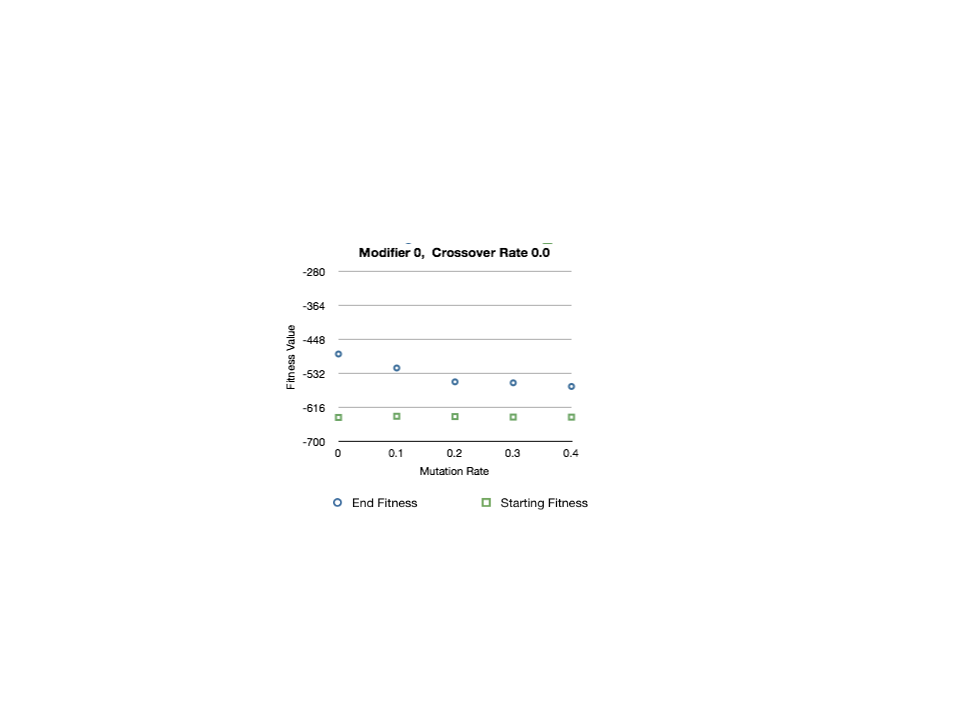
\includegraphics[width=10in]{images/FitMute00.png}\hspace*{0in}\vspace*{-2in}
	\caption{Equally weighted variables, 0.0 crossover rate fitness comparisons}
	\label{Figure 1}
\end{figure}\vspace*{-4in}


\begin{figure}[h!]
	\hspace*{-2in}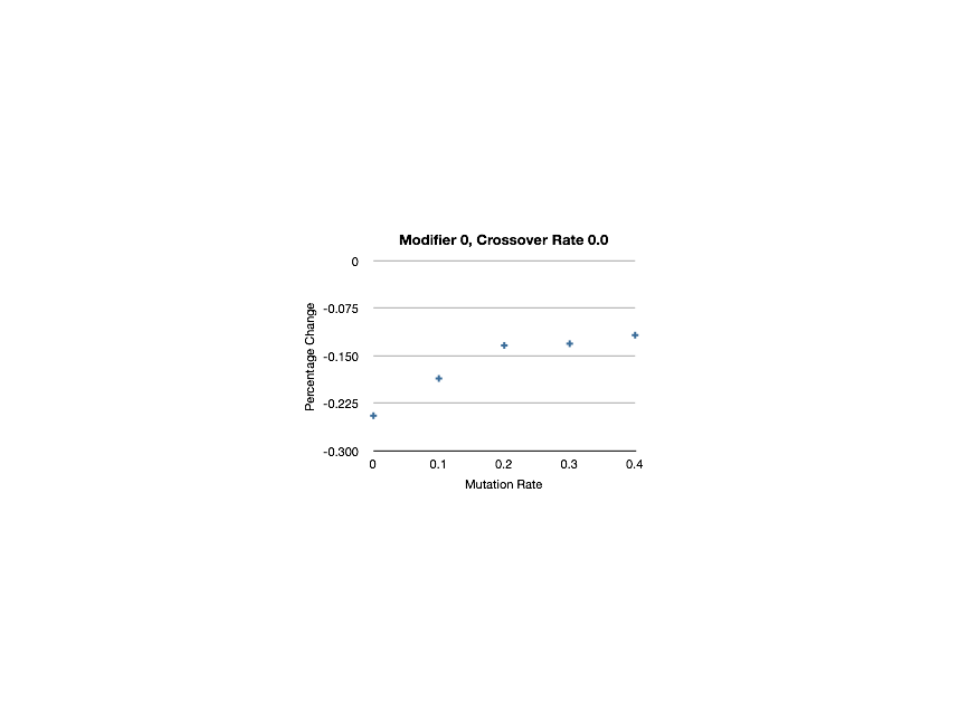
\includegraphics[width=10in]{images/FitMute00Percent.png}\hspace*{0in}\vspace*{-2in}
	\caption{Percent change between starting fitnesses and final fitnesses}
	\label{Figure 2}
\end{figure}

\newpage
It should be noted that values closer to 0 indicate a ``better" fitness level and closer to optimization, while percentage change values further from 0 indicate that a greater change happened between original fitness to final fitness.  Additionally, all of these graphs use average values of the twenty different seeds used for each trial.  This was to ensure an accurate coverage and number of repetitions were done.
\vspace*{-2in}
\begin{figure}[h!]	
	\hspace*{-2in}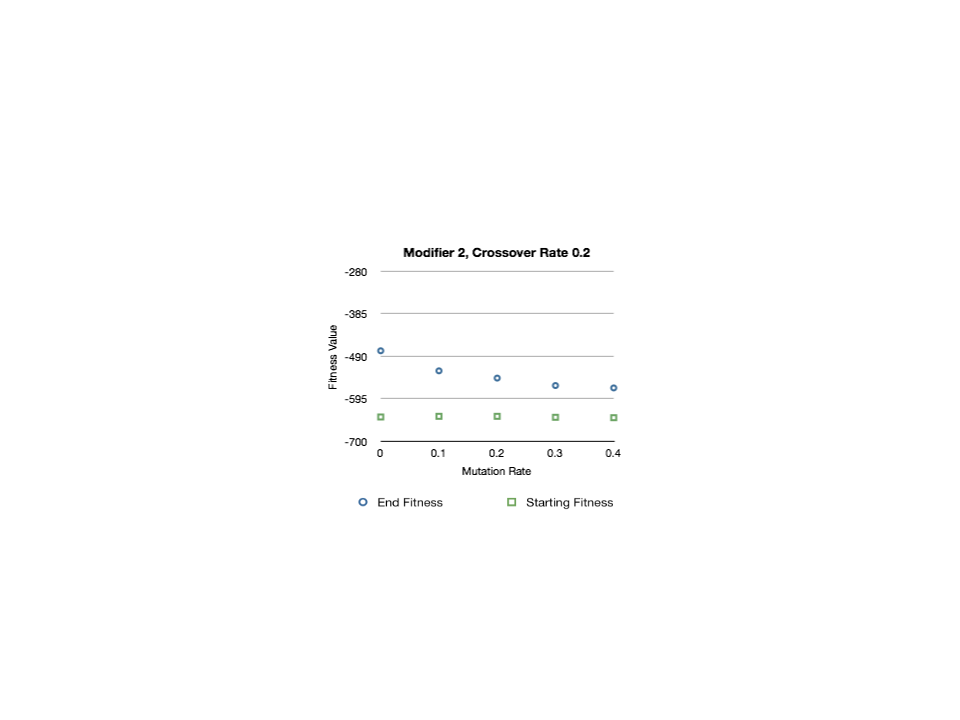
\includegraphics[width=10in]{images/FitMute02.png}\hspace*{0in}\vspace*{-2in}
	\caption{Time delay heavily weighted (.6 vs .3), 0.2 crossover rate fitness comparisons}
	\label{Figure 3}
\end{figure}

\begin{figure}[h!]	
	\hspace*{-2in}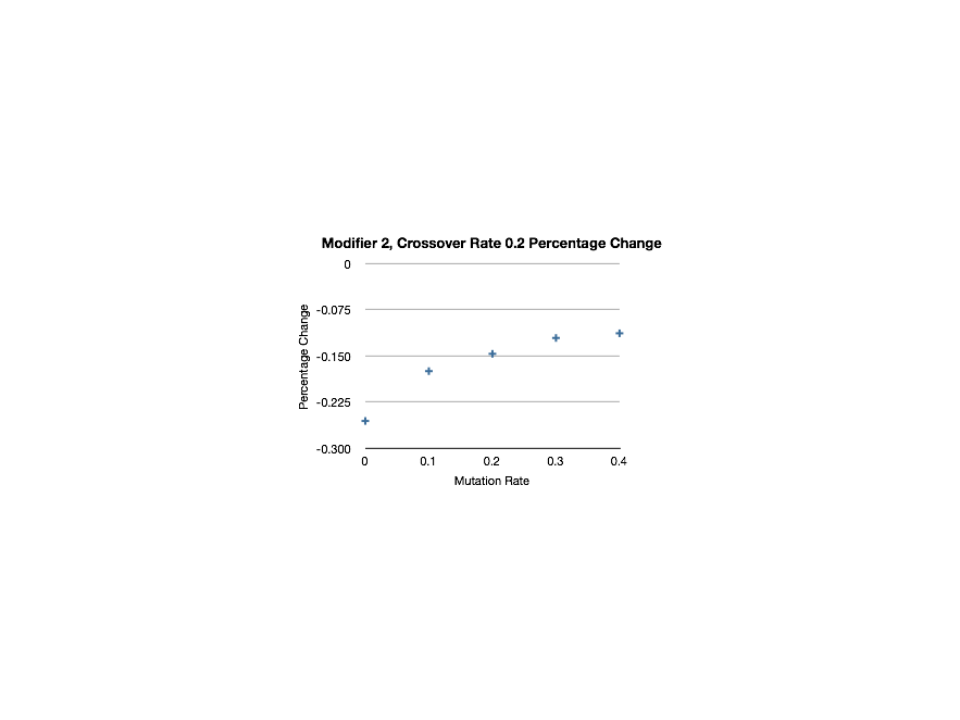
\includegraphics[width=10in]{images/FitMut02Percent.png}\hspace*{0in}\vspace*{-2in}
	\caption{Percent change between starting fitnesses and final fitnesses}
	\label{Figure 4}
\end{figure}

\begin{figure}[h!]
	\hspace*{-2in}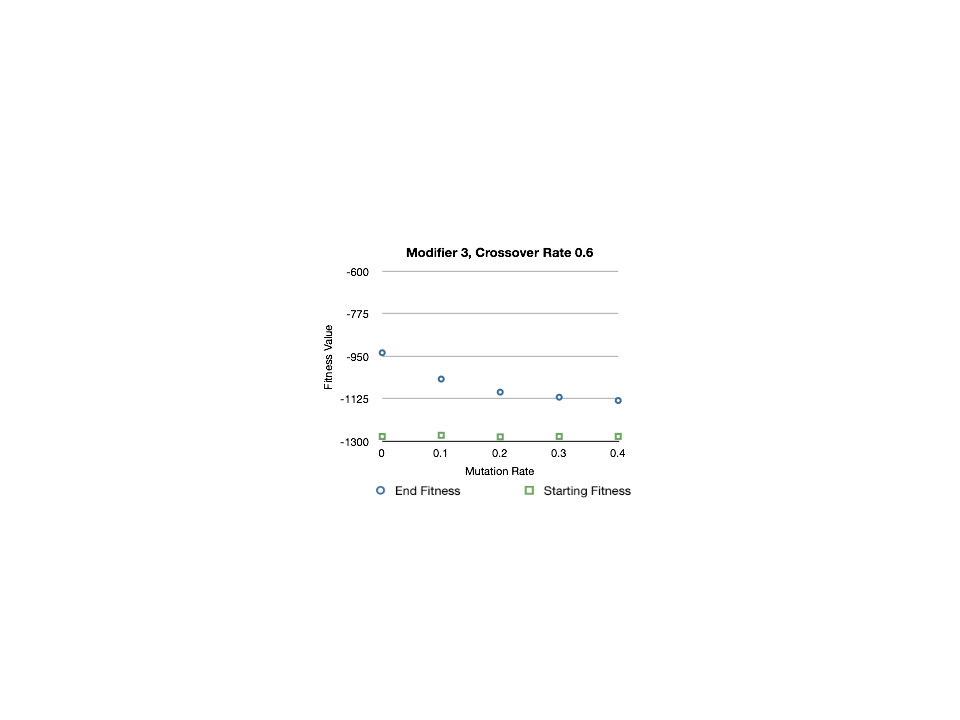
\includegraphics[width=10in]{images/FitMut03.png}\hspace*{0in}\vspace*{-2in}
	\caption{Fuel consumption heavily weighted (.6 vs .3), 0.6 crossover rate}
	\label{Figure 5}
\end{figure}

\begin{figure}[h!]
	\hspace*{-2in}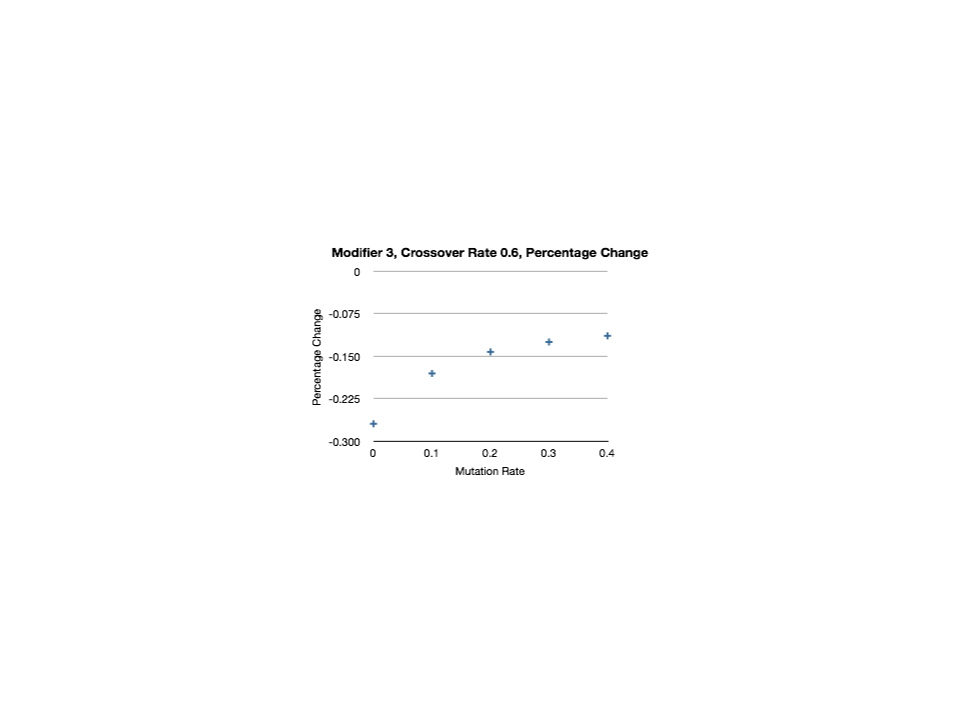
\includegraphics[width=10in]{images/FitMut03Per.png}\hspace*{0in}\vspace*{-2in}
	\caption{Percent change between starting fitnesses and final fitnesses}
	\label{Figure 6}
\end{figure}
\newpage
The precise values of the trials are as follows.  Generation number was held constant at 25 generations per trial, and population size was held at 20 individuals per generation.  Crossover probability ranged from 0.0 to 0.6, incrementing by 0.2 each iteration.  Mutation rate ranged from 0.0 to 0.5 incrementing by 0.1 each iteration.  Additionally there were four modifiers used to adjust the weight of the different criteria of the fitness function.  The weights are either all even with a multiplier value of 0.33, or one is weighted more heavily as 0.66 while the others remain 0.33.  Modifier 0 represents an even weighting, modifier 1 weighs time transit more heavily, modifier 2 weighs time delay more heavily, and finally modifier 3 weighs gas usage more heavily.  These do not seem to disrupt trend but rather appear to influence the scaling as shown in there graphs.

These results support the hypothesis that using genetic algorithms can a good metric and standard for optimizing these kind of idealized city plan systems.  This entails that genetic algorithms, or this approach to using genetic algorithms, may be appropriate to select, firstly, whether or not an intersection has a stop sign or a traffic light at each node, and secondly, the timings at each of these intersections.  This means that even though there are a myriad of variables and possible configurations, the evolutionary approach of genetic algorithms allows for the program to approach a local or global ideal state.  This is not to say that the chosen pipelines and manners in which selection and crossover were performed, could not have been improved.  For this study, the simplest of genetic algorithms was implemented using, as seen in the parameters file earlier, tournament selection, two sources for breeding, and a tournament size of two, meaning that from each generation, four random individuals were selected, and the two best of these four were used as parents for the next generation.  There are several alternatives to many of these pipelines that were used and perhaps in future studies, these may prove to perform better for this type of problem.   % Chapter organization is topic-dependent

% YOU MAY HAVE SEVERAL MORE CHAPTERS, DEPENDING ON TOPIC AND ORGANIZATION

%ch:conclusion
%
% $Id: conclusion.tex
%
%   *******************************************************************
%   * SEE THE MAIN FILE "AllegThesis.tex" FOR MORE INFORMATION.       *
%   *******************************************************************


\chapter{Discussion and Future Work}\label{ch:conclusion}

This section covers and discusses the possible field of future works, and broadly overviews and reviews some of the issues, discoveries, and information delivered by the other aspects of this paper.

\section{Summary of Results}
As mentioned before, the results of this project were relatively promising.  The system was able to optimize the traffic grid up to 35\% more than the starting fitness in some cases.  While these solutions could be more accurate with the use of a more accurate simulator, this is not a bad starting point and should encourage further research in the field.  It was also observed that several of the variables tested for performance, had little effect on the outcomes of the optimization process.  An exception was the mutation rate, where lower values resulted in greater optimization.  Finally, the only major variation in values stemmed from weighing the different variables for the fitness function differently.  Even with these variations, overall trends remained consistent.

\section{Future Work}
The most easily achievable improvement to this project would be a better representation of the map and traffic system.  This would include a more realistic map, while still constrained to the grid system, involving more accurate speed limits for these roads, car destination and starting point hot spots, a better direction choosing system, and a better method of having cars enter and exit the system.  The speed limits and car starting and destination choices would be very simple, yet time-intensive jobs.  It would entail limits within the city being set for urban, housing, and commercial sections,  better approximating the way cities exist in real life.  Concurrently, it would be beneficial for a better direction setting algorithm to be used in place of breadth-first search.  Djikstra's algorithm is a possible replacement, because it calculates weight, or the speed limit of a road in this situation, as a factor while deciding on the best path.  Finally, allowing cars to enter and exit the system at different times so that there wasn't a flood of them entering the system at once would be an improvement.  This could be achieved by keeping a global time within the system and incorporating an entrance time variable for each car.   Exiting the system in a more elegant manner would be slightly more involved and require additional variables and checking to be made for how far in a road a car was and needed to be to be considered at its destination.  Doing this in a generic way would be slightly more complex.

Besides the above simple steps for increasing the accuracy of this project's system, there are other areas which can be improved in future work.  These are primarily limited to having more accurate simulation models and using these models on more accurate real city plans.  As mentioned, the primary drawback of this study was the amount of time that could be diverted to the development of the simulator.  If the simulation were more accurate, then indications of how well the genetic algorithm is able to perform would also be much more accurate.  Enhancements towards realism would include the use of irregular sized intersections (more or less than 4 lanes), as well as factors pertaining to the characteristics and behaviors of the cars.  Additionally, incorporating aspects such as rush hour, weather, driver personalities, road construction, and other driving irregularities would render the simulator more realistic.  The simulator also, as discussed earlier, is in charge of evaluating the fitness of the configuration.  It would be interesting to see if a new fitness could be developed which was able to more accurately portray how well the traffic configuration was able to influence and improve the conditions within the system.  

A final area of future work for this project might be the comparison of this project's methods with several of the afore-mentioned algorithms in the related works section.  Although this method was able to successfully optimize systems, the degree to which they were improved could perhaps be increased through the use of other algorithms, or partial genetic algorithms which use some heuristic to avoid local minima and maxima.  Comparing the results of this algorithm, and the results of other algorithms used on the same system would provide a better idea on how well this heuristic was able to optimize the system.

\section{Conclusion}
As a review, this study had the goal of showing that genetic algorithms, when coupled with a simulator to evaluate fitness, are able to adequately optimize a traffic grid to minimize several resultants of the system.  These include time delay, total time transit, and gas usage of the cars within the system.  To do this, a simulator was built which would take a perfect square as a grid pattern, incorporate speed limits and other aspects, introduce a number of randomly or personally configured cars, and implement an intersection configuration file to run as a discrete event simulator.  The simulations eventually resulted in a fitness numbers which represented the different important values itemized earlier, that were then used to indicate how well the current light configuration performed.  This simulator was then paired with the ECJ evolutionary algorithm suite to implement a genetic algorithm which generated and eventually proposed a more optimal traffic configuration.

To test the performance of these components, an exhaustive suite of trials was run impacting the mutation rate, crossover rate, and modifier weights, related to the fitness function.  These were run through a bash script and the results compiled and analyzed.  The findings indicate that genetic algorithms and this projects approach may be a valid and powerful tool to optimizing a large traffic grid through manipulation of the intersection traffic controls only.  Additionally none of the trialed values had a major impact on the results of the trials apart from the mutation rate.  In this case, it was found that having a lower mutation rate of 0 was the most powerful.  This trend was produced across all other configurations of the genetic algorithm

This study encourages research to move further into the presented problem of optimizing traffic control configurations to minimize congestion and delays.   Implementing different genetic algorithms is suggested.  Perhaps using multi-objective genetic algorithm would yield better results.  Finally, making a comparative study between this implementation and other heuristic algorithms would allow the findings of this study to be compared with other approaches and thus result in more meaningful conclusions.   % Conclusion/future work

%   ********************************************************************
%   * IF YOU HAVE ANY APPENDICES (FOR INSTANCE, CODE, DATA, GRAPHS,    *
%   * OR ANYTHING ELSE THAT DOESN'T "FIT" AS REGULAR CHAPTER CONTENT), *
%   * INCLUDE THE FOLLOWING LINE, WHICH INSTRUCTS LATEX TO CHANGE FROM *
%   * NUMBERED "CHAPTER" HEADINGS TO LETTERED "APPENDIX" HEADINGS.     *
%   *                                                                  *
%   * APPENDICES HAVE THE SAME FORMATTING COMMANDS AS CHAPTERS (E.G.,  *
%   * "\chapter{...}", "\section{...}", ETC.)                          *
%   ********************************************************************

\appendix

%
% $Id: appa--code
%
%   *******************************************************************
%   * SEE THE MAIN FILE "AllegThesis.tex" FOR MORE INFORMATION.       *
%   *******************************************************************

\chapter{Project Code}\label{appa:code}

\section{Simulator}
\subsection{Core}
\lstinputlisting{Code/AbstractSimulator.java}
\newpage
\lstinputlisting{Code/Simulator.java}
\newpage
\lstinputlisting{Code/TrafficSimulator.java}
\newpage
\lstinputlisting{Code/AbstractEvent.java}
\newpage
\lstinputlisting{Code/Event.java}
\newpage
\lstinputlisting{Code/NodeEvent.java}
\newpage
\lstinputlisting{Code/CarEvent.java}
\newpage
\lstinputlisting{Code/RuntimeOperations.java}
\newpage

\subsection{Input/Output}
\lstinputlisting{Code/ECJPlug.java}
\newpage

\subsection{Utilities}
\lstinputlisting{Code/TrafficMap.java}
\newpage
\lstinputlisting{Code/Graph.java}
\newpage
\lstinputlisting{Code/Node.java}
\newpage
\lstinputlisting{Code/DirectionalQueue.java}
\newpage
\lstinputlisting{Code/Edge.java}
\newpage
\lstinputlisting{Code/CarObj.java}
\newpage
\lstinputlisting{Code/CarGen.java}
\newpage

\subsection{Support Files}
\lstinputlisting{Code/Cars.txt}
\newpage
\lstinputlisting{Code/Edge.txt}
\newpage
\lstinputlisting{Code/Node.txt}
\newpage

\section{ECJ Optimizer}
\lstinputlisting{Code/TrafficSim.java}
\newpage
\lstinputlisting{Code/TrafficSim.params}
\newpage

\section{Support Programs}
\lstinputlisting{Code/ParamsGen.java}


  % Appendices go here


%   ********************************************************************
%   * THE FINAL COMMANDS DEAL WITH BIBLIOGRAPHY/REFERENCES. IF THERE   *
%   * ARE ANY ITEMS IN YOUR BIBTEX FILE THAT YOU DID NOT REFERENCE IN  *
%   * YOUR PAPER, BUT THAT YOU WISH TO INCLUDE IN THE BIBLIOGRAPHY,    *
%   * YOU MAY SPECIFY "\nocite" COMMANDS TO FORCE THEM TO BE INCLUDED. *
%   *                                                                  *
%   * THE COMMAND "\nocite{*}" FORCES EVERY ITEM IN YOUR BIBTEX FILE.  *
%   ********************************************************************

%\nocite{ckm-acmap-99}   % EXAMPLES OF FORCING THINGS TO BE INCLUDED
%\nocite{Dierckx93}      %   "   "   "
%\nocite{obs-stcav-92}   %   "   "   "
%\nocite{bb4471}         %   "   "   "

\nocite{*} % OR DO THIS TO INCLUDE ALL BIBTEX REFERENCES IN THE BIBLIOGRAPHY

\bibliographystyle{plain}

%   ********************************************************************
%   * IF YOU HAVE YOUR BIBLIOGRAPHY IN A SEPARATE ".bib" FILE, HERE IS *
%   * WHERE YOU MUST SPECIFY IT. IN THIS EXAMPLE, THE BIBLIOGRAPHY     *
%   * ENTRIES ARE STORED IN A SUBDIRECTORY NAMED "Bibdir" IN A FILE    *
%   * NAMED "myBibtexDB.bib".                                          *
%   ********************************************************************

\begin{spacing}{1}
\bibliography{bib}    % File type ".bib" is assumed
\end{spacing}

%   ********************************************************************
%   * THIS FEATURE HAS BEEN DISABLED:                                  *
%   ********************************************************************
% \include{colophon}

\typeout{THEPAGE \thepage}

\end{document}
